\section*{Introduction}\label{sec:intro}

The object of these lecture notes is to provide an expository account of recent work in the study of braid varieties and their relation to low-dimensional contact and symplectic topology. A driving theme will be the development and use of Demazure weaves to construct cluster algebra structures on the coordinate rings of such braid varieties.\\

\noindent The first part of the manuscript addresses algebraic and combinatorial aspects of braid varieties building on the diagrammatic calculus of weaves. Its main goal is to explain how to use Demazure weaves to construct cluster algebra structures on the coordinate rings of braid varieties. The second part is focused on the study of Legendrian links and their Lagrangian fillings using weaves, which helps illustrate one fruitful connection between these braid varieties and their cluster structures, weaves, and symplectic topology.\\

%%%%%%%%%%%%%%%%%%%%%%%%%%%%%%%%%%%%%
%%%%%%%%%%%%%%%%%%%%%%%%%%%%%%%%%%%%%
%%%%%%%%%%%%%%%%%%%%%%%%%%%%%%%%%%%%%

\noindent {\bf Scientific context for Part I.} The study of Lie groups $\G$, their Lie algebras $\mathfrak{g}$, and their representation theory is useful in mathematics, see e.g.~\cite{MR1920389,MR2069175,MR2440737,MR3331229,MR1240056,MR1345386,MR3443860}. In many of its incarnations, it builds on the Weyl groups $W(\G)$ and the manner in which they help organize different structures around $\G$, e.g.~via the Bruhat decomposition, or by encoding symmetries of roots. Among other features, braid varieties $X(\beta)$ and their associated weave diagrams $\wb$, where $\beta\in\Br^+(W(G))$ is a positive braid word, provide new ground to explore a version of {\bf non-reduced Lie theory}, where the role of elements of the Weyl group $W(\G)$ is played by the positive braid monoid $\Br^+(W(\G))$, and that of reduced expressions for $w\in W(\G)$ is played by positive braid words $\beta=\s_{i_1}\s_{i_2}\cdot\ldots\cdot\s_{i_l}$. Some instances of this phenomenon are as follows:\\

\begin{enumerate}
    \item The intersection theory of Schubert cells in flag varieties $\G/\borel$ and Grassmannians. Historically rooted in enumerative algebraic geometry, these also naturally arise when studying the Bruhat decomposition
        \begin{equation}\label{eq:Bruhat_decomposition}\G=\bigsqcup_{w\in W}\borel w\borel
        \end{equation}
    of $\G$ and projecting to $\G/\borel$. For instance, it follows from \eqref{eq:Bruhat_decomposition} that elements in $W(\G)$ dictate the possible relative positions between two flags. Overall, if $\borel_-$ is the opposite Borel, intersections of the form
        \begin{equation}\label{eq:intersection_shape}
            \fbox{$(\borel u\borel)\cap(\borel_- v\borel_-)$}\qquad u,v\in W(\G)
        \end{equation}
and their analogues in flag varieties and Grassmannians have a central role in Lie theory and algebraic combinatorics. Double Bruhat cells, Richardson varieties, and intersections of Schubert varieties can be understood as instances of \eqref{eq:intersection_shape}, and the variants $(\borel u\borel)\cap\uni_-$ provide unipotent cells. Braid varieties $X(\beta)$ generalize these and, coarsely put, can be understood as being of the form \eqref{eq:intersection_shape} if we wrote $(\borel\beta\borel)\cap(\borel_-\delta(\beta)\borel_-)$, where we need to make rigorous sense of $\borel\beta\borel$ for a positive braid word $\beta$, and $\delta(\beta)\in W(\G)$ is the Demazure product of $\beta$, which is still an element of the Weyl group.\\

\item The coordinate rings of varieties arising as \eqref{eq:intersection_shape} tend to have remarkable combinatorial structures, central to them being the fact that they admit the structure of a cluster algebra, cf.~\cite{FWZ16,FZ2002I,FZ2003II,BFZ2005,FZ2007IV,BZ2005}. This is also the case for many of their cousins, such as the positroid subvarieties of Grassmannians, cf.~\cite{GL2023,Scott06,SSBW2019,FSB2022,JKS2016,BKM2016}. An important fact about braid varieties $X(\beta)$, proven in \cite{CGGLSS25}, and see also \cite{GalashinLamShermanBennettSpeyer2022TypeA,GalashinLamShermanBennett2026GeneralType,casals2025comparingclusteralgebrasbraid}, is that their coordinate rings $\Z[X(\beta)]$ admit the structure of a cluster algebra, and each Demazure weave $\wb$ provides a cluster seed for such a cluster algebra. It does so in an explicit manner, so that both the quiver and the cluster variables are readily computable via weaves.\\

\noindent Here the diagrammatic calculus of weaves, cf.~\cite{CasalsZaslow,CasalsWeng22,CGGJ24,CGGLSS25}, could be seen as generalizing the role played by the appropriate algebraic combinatorial objects in the reduced cases, e.g.~reduced plabic graphs in the case of positroids, or (tagged) triangulations in the case of cluster algebras associated to surfaces \cite{FG2006,FST08,FT12}. Thus an important feature of many Lie theoretic varieties, namely the existence of cluster algebra structures and diagrammatic combinatorics used to manipulate them, seems to still persist when we enter the non-reduced land through the lens of braid varieties.\\

\item Building on the introduction of global bases in representation theory, the coordinate rings of varieties of the form \eqref{eq:intersection_shape} provide fruitful soil for algebraic combinatorial models describing global bases. In particular, the classical theory of crystal bases, which captures part of the structure of such global bases, has $W(\G)$ and the roots of $\G$ as building ingredients. To wit, the Lusztig data that parametrize different crystals of interest depend on a choice of a reduced expression for a certain $w\in W(\G)$, depending on the coordinate ring being studied. In line with this, the monoidal categorification of cluster coordinate rings of varieties of the form \eqref{eq:intersection_shape}, where such a ring is realized as a Grothendieck ring $K_0$ of a monoidal category, was pioneered by D.~Hernandez and B.~Leclerc, cf.~\cite{MR2682185,MR3077685,MR3331727,MR3500832,MR3576119,MR4404353}.\\

In the non-reduced case of braid varieties $X(\beta)$, monoidal categorifications have recently been constructed and their corresponding theory of global bases and crystals is now rather well-established thanks to the work of M.~Kashiwara and his co-authors, cf.~\cite{KangKashiwaraKimOh2018Monoidal,KKOP2020Monoidal,KKOP2024MonoidalII,KKOP2025MonoidalIII,KKOP2024PBWAffine,KashiwaraPark2022CategoricalCrystals,Park2023ExtendedCrystals,OhPark2025BosonicPBW,KKOP2025GlobalBases,KKOP2024BraidSymmetries,KKOP2025Faithful} and see also \cite{Bi2026Quantization,Bi2026TwistedProducts,HuhJungKimPark2026Comparison}. In particular, there is a precise sense in which the classical $w$-Lusztig data, with $w\in W(\G)$, can now be generalized to $\beta$-Lusztig data, where $\beta$ is a positive braid word. The two key ingredients to make sense of this non-reduced version of Lusztig data are the extended crystal $\widehat{B}(\infty)$ and the braid group symmetries that they construct on the monoidal category, the extended crystal $\widehat{B}(\infty)$, and their associated objects, including the bosonic extension algebra, which in a sense contains $\Z[X(\beta)]$ for all positive braid words $\beta$.\\

\item The additive categorification of coordinate rings of varieties of the form \eqref{eq:intersection_shape} leads to a rich interplay between the classical tilting theory for Abelian categories of modules, e.g.~over preprojective algebras, and the combinatorics of quiver mutation and cluster variables, see e.g.~\cite{MR2242628,GLS08,GeissLeclercSchroer2013QuantumCoordinate,MR3534832} and \cite{JKS2016,BKM2016,MR3694688,MR4662273,MR4456104,MR2844757}. In addition to providing enlightening results on the representation theory of quivers (and their potentials, see \cite{DWZ08,DWZ10_2}), these additive categorifications nicely interact with classical structures from Lie theory, such as highest weight structures, cf.~\cite{CPS88,Kra17,BS24}. While highest weight structures were in part motivated by the study of Verma modules and the representation theory of the Lie algebras $\mathfrak{g}$, they naturally appear when additively categorifying the cluster algebras for the coordinate rings of varieties of the form \eqref{eq:intersection_shape}, see e.g.~\cite{IR11} and \cite{MR2242628,GLS08,BIRS09}.\\

We have now recently established in \cite{CasalsChrist} the non-reduced generalization of such additive categorifications for braid varieties $X(\beta)$ and their Demazure weaves. A key fact is that non-reducedness naturally leads to considering derived categories, rather than just their Abelian hearts.\footnote{Or more generally, pretriangulated dg categories, or stable $\infty$-categories, which is the viewpoint in \cite{CasalsChrist}.} An important feature of these additive categorifications of braid varieties $X(\beta)$ is the emergence of a derived analogue for highest weight theory, with full exceptional collections acquiring the role of standard objects. The role of universal extensions and quotients is now played by a truncated version of spherical twist functors, which allow for the construction of both simple-minded and silting collections from the exceptional collection, much in line with how simple and indecomposable projective objects are classically built from standard objects. In short, we have a glimpse of the non-reduced world and see how important categorical results and theories in the Abelian (reduced) setting seem to be part of, and sometimes better understood via, a derived (non-reduced) theory based on the positive braid monoid.\\

    \item Seeded in G.~Lusztig's study of positivity for reductive Lie groups \cite{Lusztig,Lusztig1997PositivityBases,Lusztig1998,Lusztig2019PositivityII,Lusztig2025Survey}, positive structures are starting to have a more unified theory around them. Examples include the positivity phenomena for cluster algebras \cite{FZ1999,Fomin2010,FominLusztig2022,FZ2000Tests,BFZ1996,BZ1997,LS2015,MSW2011,Davison2018,DM2021}, the positive representations in higher Teichm\"uller theory \cite{FG2006,MR2221137}, positive geometries \cite{ABL2017,ABHY2018,ALS2021,Lam2024Invitation,Lam2025Moduli}, and positivity in matroids \cite{ARW2017}, see also \cite{KW2014}. Varieties appearing as \eqref{eq:intersection_shape} do exhibit such positivity, e.g.~existence of a positive atlas, and positive properties for some of their global bases, cf.~G.~Lusztig's works above. Such positivity features are also shared by braid varieties $X(\beta)$, see e.g.~\cite{BaoHe2022TwistedPositivity}. These positivity properties have an important role when discussing tropicalization and parametrizing global bases. In the context of Demazure weaves, even the most basic definitions, such as those of Lusztig cycles and their associated quiver, are grounded on tropical identities arising from this underlying positivity.\\
\end{enumerate}

\noindent The above are a few instances of this reduced to non-reduced phenomenon, selected just from personal knowledge. See also \cite{trinh2021heckecategoryunipotentlocus,trinh2022unipotentelementstwistinglink} for another interesting example, where identities of R.~Steinberg \cite[Theorem 15.1]{Steinberg1968Endomorphisms} and N.~Kawanaka \cite[Theorem 4.1]{Kawanaka1975} on certain counts over finite fields in the reduced setting are enhanced to $\ell$-adic cohomological isomorphisms and established in the braid variety non-reduced setting, cf.~\cite[Corollary 4]{trinh2021heckecategoryunipotentlocus} and see also \cite[Conjectures 1 \& 17]{trinh2022unipotentelementstwistinglink}. It should be emphasized that there are many previous works that point toward such non-reduced extensions in and around Lie theory. These include works of P.~Deligne, G.~Lusztig and others, see e.g.~\cite{Deligne1972Tresses,Deligne1997Action,DeligneLusztig1976Representations,BroueMichel1997Regular,DigneMichelRouquier2007Cohomologie,Lusztig2011Varieties} and cf.~\cite[Appendix B]{trinh2021heckecategoryunipotentlocus}. Note as well that varieties that arise by considering (not necessarily reduced) positive braid words have also a prominent standing in geometry and topology, see \cite{Bott1956Morse,BottSamelson1958Morse,Demazure1974Desingularisation,LakshmibaiLittelmannMagyar2002SMT} and the second part of these notes, especially its relation to \cite{FG2006}.

\begin{table}[h!]
  \centering

\begin{tabular}{ |P{4cm}|P{5cm}|P{5cm}|}
	\hline
     & {\bf Reduced expression $w\in W(\G)$} & {\bf Positive braid word $\beta\in\on{Br}^+(W(\G))$}\\
	\hline

    Algebraic variety & $(\borel u\borel)\cap(\borel_- v\borel_-)$ & $X(\beta)\approx(\borel \beta\borel)\cap(\borel_- \delta(\beta)\borel_-)$\\
	\hline

    \rule{0pt}{0.5cm}Coordinate ring & Cluster algebra & Cluster algebra\\
	\hline

    \rule{0pt}{0.5cm} Some algebraic combinatorial objects & double wiring diagrams, plabic graphs, and more & Demazure weaves $\wb$\\
	\hline

    \rule{0pt}{0.5cm} Positive global bases and crystals & canonical bases and $w$-Lusztig data & canonical bases and $\beta$-Lusztig data\\
	\hline

    \rule{0pt}{0.5cm}Constructing additive categorifications & Via simples and tilting in an Abelian category & Simple-minded and silting in derived category\\
	\hline

    \rule{0pt}{0.5cm}Constructing monoidal categorifications & Via subcategories of $\mathcal{U}_q'(\widehat{\mathfrak{g}})$-mod& By incorporating braid group action and symmetries\\
    \hline
\end{tabular}
  \caption{Summary of analogies between objects and results when using a reduced expression for an element $w\in W(\G)$ of the Weyl group, and their putative counterparts when using a (not necessarily reduced) positive braid word $\beta\in\Br^+(W(\G))$.}  \label{table:summary_nonreduced}
\end{table}
\vspace{0.1cm}

\noindent The comments above are summarized in Table \ref{table:summary_nonreduced}. There are many additional aspects to Table \ref{table:summary_nonreduced} that are unfortunately omitted, e.g.~the work of B.~Keller, C.~Amiot, Y.~Wu and others on cluster and Higgs categories, see e.g.~\cite{MR2640929,amiot2011generalizedclustercategories,MR2764906,MR3024264,MR4289034,MR4157113,MR2762547,Keller12_DT2,MR2795754,MR2385670,MR2316979,MR4581969,MR4576399}, for the row on additive categorifications, or the work of P.~Galashin, T.~Lam, M.~Sherman-Bennett and D.~Speyer on 3D plabic graphs \cite{GalashinLamShermanBennettSpeyer2022TypeA} for another instance of Type A combinatorics for non-reduced $\beta$.\footnote{I apologize for other involuntary sins of omission: should the reader think a citation to another work must be added, please contact the author.} The content of these notes will focus on the study and construction of cluster algebras in and around braid varieties, i.e.~$(1)$ and $(2)$ above. Items $(3)$ and $(4)$, and in a sense $(5)$, require an understanding of such cluster structures in $(2)$, and thus it seems appropriate to focus on $(2)$ for now.\\

%%%%%%%%%%%%%%%%%%%%%%%%%%%%%%%%%%%%%
%%%%%%%%%%%%%%%%%%%%%%%%%%%%%%%%%%%%%
%%%%%%%%%%%%%%%%%%%%%%%%%%%%%%%%%%%%%
\noindent {\bf Main Results related to Part I.} Let $\G$ be a simple algebraic Lie group and $\beta\in\Br^+(\G)$ a positive braid word. The first part of these notes focuses on the combinatorial and algebraic aspects of braid varieties $X(\beta)$, \cite{CGGJ24,CGGLSS25} and see \cite[Appendix B]{trinh2021heckecategoryunipotentlocus}. Intuitively, the points in the algebraic varieties $X(\beta)$ parametrize linear tuples of flags in $\G/\borel$ in certain relative positions. The relative positions are given by the crossings, i.e.~the letters, of the positive braid word $\beta$. Specifically, let $\beta = \sigma_{i_1}\cdots \sigma_{i_{\ell}}$ be a positive braid word and $\delta(\beta) \in W(\G)$ its Demazure product. By definition, the {\it braid variety} associated with $\beta$ is
\begin{equation}\label{eq:braid_variety}
X(\beta) := \{(\borel_1, \dots, \borel_{\ell+1}) \in (\G/\borel)^{\ell + 1} \mid \borel_1 = \borel, \borel_{k} \buildrel s_{i_{k}} \over \longrightarrow \borel_{k+1}, \borel_{\ell + 1} = \delta(\beta) \borel \},
\end{equation}
\noindent where $\delta(\beta) \in W(\G) \cong N_{\G}(\T)/\T$ has been lifted to $N_{\G}(\T)$. These are studied in detail in \Cref{sec:weaves_braid_varieties}. In particular, they are smooth irreducible varieties over $\Z$ and their isomorphism type only depends on the underlying braid element $[\beta]\in\B(\G)$.

\begin{center}
	\begin{figure}[h!]
		\centering
		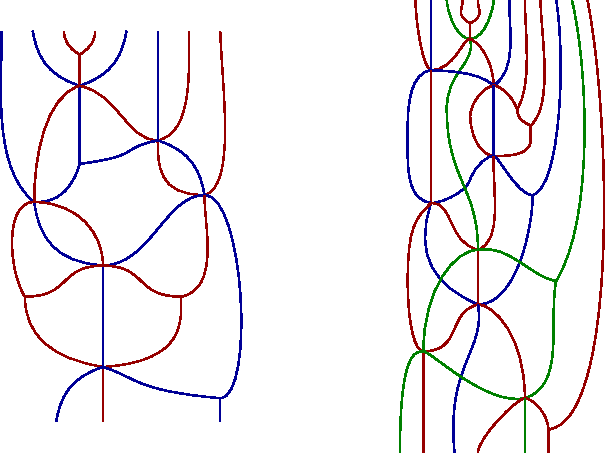
\includegraphics[scale=1]{figures/Example_TwoWeavesSL3SL4.pdf}
		\caption{Two instances of Demazure weaves. These diagrams are read top-to-bottom, and can be intuitively understood as ways to simplify a positive braid word $\beta$, starting at the top, down to a permutation, at the bottom. (Left) A Demazure weave $\w:\beta\lr\delta(\beta)$ in $\SL_3$, from the 3-stranded braid word $\beta=\s_1^2\s_2^2\s_1^2\s_2^2$ to $\delta(\beta)=\s_1\s_2\s_1$, where blue weave edges are labeled by $\s_1\in S_3$ and red weave edges by $\s_2\in S_3$. (Right) A Demazure weave $\w:\beta\lr\delta(\beta)$ in $\SL_4$, from the 4-stranded braid word $\beta=\s_2\s_1\s_3\s_2^2\s_1\s_2^2\s_1\s_3\s_2$ to its Demazure product $\delta(\beta)$, where blue weave edges are labeled by $\s_1\in S_3$, and red and green weave edges by $\s_2$ and $s_3\in S_4$ respectively.}
		\label{fig:Example_TwoWeavesSL3SL4}
	\end{figure}
\end{center}

A central contribution of Part I is to develop the diagrammatic calculus of Demazure weaves, which provides an algebraic and combinatorial framework to study the geometry of $X(\beta)$ and the algebraic properties of its coordinate ring of regular functions $\Z[X(\beta)]$. \Cref{fig:Example_TwoWeavesSL3SL4} depicts two instances of Demazure weaves for $\G=\SL_3$ and $\SL_4$. In a nutshell, a Demazure weave $\wb$ is a specific sequence that simplifies a positive braid word $\beta$ to its Demazure product $\delta(\beta)$ by using either braid moves, which contribute to 4 and 6-valent vertices, or the operation $\s_i^2\to\s_i$, which contributes a trivalent vertex. We will introduce the notion of weave equivalences, which generalize relations between syzygies in the positive braid monoid, and the operation of weave mutation.

\begin{table}
\begin{center}
\caption{Some of the concepts being studied in Part I.}\label{table:PartI_introduction}
\small
\begin{tabular}{ |P{3.8cm}|P{5.5cm}|P{4.8cm}|  }
	\hline
	\multicolumn{3}{|c|}{ {\bf First algebraic and combinatorial aspects of Demazure weaves}} \\
	\hline

{\bf Weaves} & {\bf Braid varieties} & {\bf Cluster theory}\\
\hline

Positive braid word $\beta$ & Algebraic variety $X(\beta)$ & Cluster algebra $\Z[X(\beta)]$\\
\hline
Demazure weave $\w:\beta\to\delta(\beta)$ & Open embedding of algebraic torus $\iota_w:T_\w\hookrightarrow X(\beta)$ & Chart morphism $\Z[X(\beta)]\to\Z[u_1^{\pm1},\ldots,u_r^{\pm1}]$\\
\hline
Lusztig cycles $\{\g_v\}$ & Rational functions $X^\w_v\in\Z(X(\beta))$ & cluster $\SX$-variables $\{X_v^\w\}$\\
\hline
Dual Lusztig cycles $\{\r_v\}$ & Regular functions $A^\w_v\in\Z[X(\beta)]$ & cluster $\SA$-variables $\{A_v^\w\}$\\
\hline
Intersecting weave cycles & Algebraic 2-form $\omega_{cl}\in\Gamma(T_\w,\Omega^2 T_\w)$ & Quiver $Q_\w$\\
\hline
Weave mutation $\w\stackrel{\mu}{\sim}\w'$ & Change of torus $\iota_\w(T_\w)\neq \iota_{\w'}(T_{\w'})$ & Cluster mutation\\
\hline
\end{tabular}
\normalsize
\end{center}
\end{table}



\begin{comment}

\begin{enumerate}
    \item Any pair of Demazure weaves $\wb$ can be connected by a sequence of weave equivalences and weave mutations.\\
    \item The intersection theory of Lusztig cycles and dual Lusztig cycles of a Demazure weave $\wb$ is invariant under weave equivalences, and it changes according to quiver mutation for weave mutations.\\
    
    \item A Demazure weave $\wb$ provides a cluster $\SA$-seed $(T^\SA_\w,Q_\w,\{A_i^\w\})$ so that $A_i^\w\in\Z[X(\beta)]$, $Q_\w$ encodes the intersections of dual Lusztig cycles, and we have an isomorphism
    \begin{equation}\label{eq:braid_variety_is_cluster}
        \Z[X(\beta)]\cong\SA(Q_\w)
    \end{equation}
    where $\SA(Q_\w)$ denotes the cluster algebra associated to the quiver $Q_\w$.\\

    \item Similarly, a Demazure weave $\wb$ provides a cluster $\SX$-seed $(T^\SX_\w,Q_\w,\{X_i^\w\})$ so that $X_i^\w\in\Z(X(\beta))$, $Q_\w$ encodes the intersections of Lusztig cycles, and $X(\beta)$ is isomorphic to the cluster $\SX$-scheme associated to $Q_\w$.\\
    
    \item Several geometric features of $X(\beta)$, including a defining ideal, a torus action and a cyclic symmetry, an algebraic closed $2$-form compatible with the cluster structures, and a natural Landau-Ginzburg potential associated to a positive braid word $\beta$, can all be expressed explicitly in terms of Reeb coordinates of $X(\beta)$.\\
\end{enumerate}
\end{comment}

From a Demazure weave $\wb$, we will explain how to construct a number of combinatorial objects, including its Lusztig cycles, its dual Lusztig cycles, and an intersection theory for them. In particular, we will obtain a quiver $Q_\w$ for each Demazure weave $\wb$, which encodes the intersections between Lusztig cycles. The vertices of the quiver are indexed by the trivalent vertices of $\w$, i.e.~one for each time we applied the operation $\s_i^2\to\s_i$ when simplifying $\beta$ to $\delta(\beta)$. The first combinatorial properties of these Demazure weaves are as follows:

\begin{fthm}\label{thm:weave_intro1}
Let $\beta\in\brn$ be a positive braid word. Then the following hold:

\begin{enumerate}[label=$(\arabic*)$]
    \item Two Demazure weaves $\w,\w':\beta\lr\delta(\beta)$ are connected by a sequence of weave equivalences and weave mutations.\\

    \item If $\w_1\simeq\w_2$ is a weave equivalence, the two intersection quivers $Q_{\w_1}$ and $Q_{\w_2}$ encoding the intersections of Lusztig cycles for $\w_1$ and $\w_2$ coincide, i.e.~$Q_{\w_1}=Q_{\w_2}$ after relabeling vertices. The same holds for the dual Lusztig cycles.\\

    \item If $\w_1\stackrel{\mu}{\sim}\w_2$ is a weave mutation at the Lusztig cycle $\gamma_{v_k}$ of $\w_1$, then the intersection quiver $Q_{\w_2}$ is obtained from $Q_{\w_1}$ by quiver mutation at its $k$th vertex, i.e.~$Q_{\w_2}=\mu_k(Q_{\w_1})$. The same holds for the dual Lusztig cycles.\\
\end{enumerate}
\end{fthm}
\vspace{0.2cm}
\noindent From a Demazure weave $\wb$, we will also construct a number of objects related to the braid variety $X(\beta)$, including an open torus chart $T_\w\sse X(\beta)$, and several functions on $X(\beta)$. This is summarized in Table \ref{table:PartI_introduction}. An important instance of this is the construction of a rational function $A_v\in\Z(X(\beta))$ for each trivalent vertex of a Demazure weave $\w$. In a nutshell, the first key results regarding cluster algebras on braid varieties can be summarized as follows.

\begin{fthm}\label{thm:cluster_variables_weave_intro2}
Let $\beta\in\brn$ be a positive braid word, $X(\beta)$ its braid variety and $\w:\beta\lr\delta(\beta)$ a Demazure weave with $d$ trivalent vertices $v_1,\ldots,v_d$. Then the following hold:

\begin{enumerate}[label=$(\arabic*)$]
    \item For every trivalent vertex $v\in\w$, the rational function $A_v\in\Z(X(\beta))$ is a regular function. That is, $A_v\in\Z[X(\beta)]$, so $A_v:X(\beta)\lr\mathbb{A}^1_\Z$ has no poles.\\

    \item For every trivalent vertex $v\in\w$, the rational function $A_v\in\Z[X(\beta)]$ is non-vanishing if and only if there is a non-vanishing weight for the Lusztig cycle $\g_v$ at an edge of the south boundary of $\w$.\\

    \item The restrictions of $A_{v_1},\ldots,A_{v_d}$ to the weave torus $T_\w\sse X(\beta)$ are a coordinate system, i.e.~
    $$T_\w\cong \Spec\Z[A_{v_1}^{\pm1},\ldots,A_{v_d}^{\pm1}].$$
    That is $T_\w\sse X(\beta)$ is cut-out as an open subvariety as the non-vanishing of all the regular functions $A_{v_i}$.\\

    \item If $\w_1\simeq\w_2$ is a weave equivalence, the two sets of regular functions $\{A^{\w_1}_{v_1},\ldots,A^{\w_1}_{v_d}\}$ and $\{A^{\w_2}_{v_1},\ldots,A^{\w_2}_{v_d}\}$ coincide.\\

    \item If $\w_1\stackrel{\mu}{\sim}\w_2$ is a weave mutation at the Lusztig cycle $\gamma_{v_k}$ of $\w_1$, then $A^{\w_1}_{v_i}=A^{\w_2}_{v_i}$ if $i\neq k$ and
    \begin{equation}\label{eq:cluster_mutation_weave_variables}
        \displaystyle A^{\w_1}_{v_k}A^{\w_2}_{v_k}=\prod_{\langle \g_i,\g_k\rangle>0} (A^{\w_1}_{v_i})^{\langle \g_i,\g_k\rangle}+\prod_{\langle \g_i,\g_k\rangle<0} (A^{\w_1}_{v_i})^{-\langle \g_i,\g_k\rangle}.
    \end{equation}

    \item There exists an isomorphism
    \begin{equation}\label{eq:braid_variety_is_cluster2}
        \Z[X(\beta)]\cong\SA(Q_\w)
    \end{equation}
    where $\SA(Q_\w)$ denotes the cluster algebra associated to the quiver $Q_\w$. In addition, the tuple $(Q_\w,T_\w,\{A^{\w}_{v_1},\ldots,A^{\w}_{v_d}\})$ is a cluster seed. In particular, any two Demazure weaves for $\beta$ provide two cluster seeds for the same cluster algebra structure in \eqref{eq:braid_variety_is_cluster2}.\\
\end{enumerate}
\end{fthm}
\vspace{0.2cm}

In particular, a Demazure weave $\wb$ provides a cluster $\SA$-seed $(T^\SA_\w,Q_\w,\{A_i^\w\})$ so that $A_i^\w\in\Z[X(\beta)]$, and $Q_\w$ encodes the intersections of dual Lusztig cycles. Similarly, a Demazure weave $\wb$ also provides a cluster $\SX$-seed $(T^\SX_\w,Q_\w,\{X_i^\w\})$ so that $X_i^\w\in\Z(X(\beta))$, $Q_\w$ encodes the intersections of Lusztig cycles, and $X(\beta)$ is the affinization of the cluster $\SX$-scheme associated to $Q_\w$. See \Cref{ssec:A_and_X_schemes_weave} for details on the relation between the cluster $\SA$ and $\SX$-schemes and $X(\beta)$.\\

\noindent We also discuss additional results, including the introduction of Reeb coordinates for $X(\beta)$. For instance, several geometric features of $X(\beta)$, including a defining ideal, a torus action and a cyclic symmetry, an algebraic closed $2$-form compatible with the cluster structures, and a natural Landau-Ginzburg potential associated to a positive braid word $\beta$, can all be expressed explicitly in terms of Reeb coordinates of $X(\beta)$. The goal of Part I of these notes is to provide the necessary details and scientific context for all these notions and results above.\\

%%%%%%%%%%%%%%%%%%%%%%%%%%%%%%%%%%%%%
%%%%%%%%%%%%%%%%%%%%%%%%%%%%%%%%%%%%%
%%%%%%%%%%%%%%%%%%%%%%%%%%%%%%%%%%%%%
\noindent {\bf Related themes for Part I.} There are different paths forward building on Theorems \ref{thm:weave_intro1} and \ref{thm:cluster_variables_weave_intro2} above. Some of them are discussed in the notes, such as studying Poisson brackets and closed 2-forms as in the work of M.~Gekhtman, M.~Shapiro and A.~Vainshtein, cf.~\cite{GSV,GSV05}, the natural superpotentials associated to a positive braid word, cf.~\Cref{thm:superpotential_Reeb_coordinates}, and finding combinatorial expansion formulas and tropical coordinates for cluster variables in terms of a given weave. The lecture notes do not discuss other equally interesting lines of continuing research. A few of these include:\\

\begin{enumerate}
    \item The combinatorial study of quivers $Q_\w$ associated to Demazure weaves $\w:\beta\lr\delta(\beta)$. It is proven in \cite{CGGLSS25} that these quivers admit reddening sequences and the associated cluster algebras are locally acyclic. But, for instance, it remains open to understand whether these quivers $Q_\w$ are either Banff or Louise.\\

    \item The additive categorification of the cluster algebra $\Z[X(\beta)]$ using weaves. This has been achieved in \cite{CasalsChrist} by constructing a perverse schober $\mathcal{F}_\w$ for each Demazure weave, and using its category of global sections $R\Gamma(\mathcal{F}_\w)$. The details of the comparison with the more classical additive categorifications in the reduced case, see e.g.~\cite{MR2242628}, are the subject of ongoing work. In particular, there is a number of interesting new structures, from the categorical and homological viewpoint, that arise when considering such categorifications, cf.~Table \ref{table:intro_homological}. A salient instance is the use of semi-twists $T^{\pm,\geq0}$ appearing as:
$$T^{+,\geq 0}_Y(X)\coloneqq \on{cof}(\tau_{\geq 0}(\on{Mor}(Y,X))\otimes Y\to X)$$
$$ T^{-,\geq0}_Y(X)\coloneqq \on{fib}(X\to \tau_{\geq0}(\on{Mor}(X,Y)^*)\otimes Y),$$
which can be understood as truncated versions of the more standard (often spherical) twists. These semi-twists preserve rigidity, behave remarkably well in the derived categorical setting, and seem to categorically capture some of the key properties of cluster algebras. The diagrammatic calculus of Demazure weaves provides an abundance of interesting examples where simple-minded collections, silting collections and their associated cluster tilting objects can be manipulated and understood in terms of weave diagrams.\\

    \item The monoidal categorification of the cluster algebra $\Z[X(\beta)]$ using weaves. In a sense, this has been partially achieved for double inductive weaves in \cite{KKOP2025MonoidalIII,Bi2026Quantization,HuhJungKimPark2026Comparison}. The general case is ongoing work, especially in relation to general Demazure weaves and $\beta$-Lusztig data.\\

    \item A systematic study of positivity aiming to address braid varieties $X(\beta)$ has been started in \cite{BaoHe2022TwistedPositivity}. A precise identification of Lusztig cycles and their duals as tropical points, building on a positive $\R_{\geq0}$-atlas still remains to be explored.\\
\end{enumerate}
In general, as hinted in the scientific context above, the established results and ongoing work seem to point towards a rather well-structured combinatorial and algebraic theory in and around braid varieties $X(\beta)$, as a non-reduced generalization of many classical Lie theoretic results. It is perhaps a sign of health for a topic in a conference titled {\it Current developments in Mathematics} that some of its natural follow-ups continue to develop, though that prevents us from providing detailed accounts of them for the time being.\\

\small
\begin{table}[htbp]
  \centering
  \caption{Homological objects featuring in the additive categorification of the cluster algebra $\Z[X(\beta)]$. Among other consequences, the existence of such structures in the derived setting hints towards a derived analogue for highest weight structures in Abelian categories.}\label{table:intro_homological}
\begin{tabular}{ |P{3cm}|P{5cm}|P{4cm}|P{5cm}|}
	\hline
    
	{\bf Highest weight abelian category} & {\bf stable $k$-linear $\infty$-category} & {\bf Expression from $(\Delta_1,\ldots,\Delta_m)$} & {\bf Categorical weave calculus for $R\Gamma(\mathcal{F}_\w)$}\\
	\hline

    standard objects & exceptional collection $\{\Delta_i\}$ & $\Delta_i$ & right weave thimbles\\
	\hline

    \rule{0pt}{0.5cm}costandard objects & coexceptional collection $\{\nabla_i\}$ & $T_{\Delta_1}^+T_{\Delta_2}^+\cdots T_{\Delta_{i-1}}^+(\Delta_i)$ & left weave thimbles\\
	\hline

    \rule{0pt}{0.5cm}simples $S_i$ & simple-minded collection & $T_{\Delta_{1}}^{+,\geq 0}(\cdots (T_{\Delta_{i-1}}^{+,\geq 0}(\Delta_i)))$ & Categorical Lusztig cycles\\
	\hline

    \rule{0pt}{0.5cm}projectives $P_i$ & first silting collection & $T_{\Delta_{m}}^{-,>0}(\cdots (T_{\Delta_{i+1}}^{-,>0}(\Delta_i)))$ & Left-dual categorical cycles\\
    \hline

    \rule{0pt}{0.5cm}injectives $I_i$ & second silting collection & $T_{\nabla_{m}}^{+,<0}(\cdots (T_{\nabla_{i+1}}^{+,<0}(\nabla_i)))$ & Right-dual categorical cycles\\
    \hline

    \rule{0pt}{0.5cm}tilting objects $T_i$ & Ringel dual silting collection & $T^{+,<0}_{\Delta_{m}^{\uparrow}}(\dots (T^{+,<0}_{\Delta_{i+1}^{\uparrow}}(\Delta_i^{\uparrow})))$ & Upward-type Lusztig cycles\\
    \hline
\end{tabular}
\end{table}
%\vspace{0.2cm}
%\noindent\rule{\linewidth}{0.4pt}
\vspace{0.5cm}
\normalsize
%%%%%%%%%%%%%%%%%%%%%%%%%%%%%%%%%%%%%
%%%%%%%%%%%%%%%%%%%%%%%%%%%%%%%%%%%%%
%%%%%%%%%%%%%%%%%%%%%%%%%%%%%%%%%%%%%
\noindent {\bf Scientific context for Part II.} For the Lie group $\G=\SL_n$, and more generally Type A, both braid varieties and Demazure weaves have a geometric model. In fact, this geometric model historically led to the systematic development of weave calculus for any simple algebraic Lie group $\G$, see \cite{CasalsZaslow,CasalsWeng22}. Specifically, for $\G=\SL_n$, a positive braid word $\beta\in\Br^+(\SL_n)$ can be used to construct a Legendrian link $\La_\beta\sse(\R^3,\xi_\std)$, see \Cref{ssec:Legendrian_link_beta}. Such a Legendrian link is a smooth link $\La_\beta\sse\R^3$ which is tangent to a certain 2-plane field, i.e.~to the contact structure $\xi_\std$.\\

A central problem in low-dimensional contact and symplectic topology is the classification of Lagrangian surfaces. In particular, given such a Legendrian link $\La_\beta\sse(\R^3,\xi_\std)$ associated to $\beta$, it is interesting and useful to try to classify all Lagrangian surfaces in $(\D^4,\la_\std)$ whose boundary is fixed to be $\La_\beta$. In precise terms, we aim at classifying all embedded exact Lagrangian surfaces $L\sse(\D^4,\la_\std)$ such that $\dd L\sse\La_\beta$, up to compactly supported Hamiltonian isotopy. These surfaces are often referred to as the Lagrangian fillings of $\La_\beta$, see \Cref{ssec:Lagrangian_fillings}. There is a rich literature constructing invariants for Lagrangian fillings, ranging from numbers to dg algebras and $A_\infty$-categories. To wit, the ruling polynomial of $\La_\beta$ \cite{Rutherford11_HOMFLY,Rutherford06_HOMFLY}, the Legendrian contact dg algebra of $\La_\beta$ \cite{Chekanov,EtnyreNg22_Survey}, similarly the partially wrapped Fukaya category stopped at $\La_\beta$ \cite{GPSCV,GPS18,Syl19}, or the dg category of sheaves with singular support on $\La_\beta$ \cite{KashiwaraSchapira_Book,GKS_Quantization,MR4612528,STZ2017}, are instances of reasonably effective invariants that aim at understanding which Lagrangian surfaces $L$ can bound a given Legendrian link $\La_\beta$. As an example of their relation to braid varieties, see \Cref{ssec:braid_varieties_Legendrian_links}, there exists an isomorphism 

\begin{equation}\label{eq:intro_braid_variety_DGA}
    \Z[X(\beta)]\cong\hH_0(\mathbb{A}^{ab}(\La_\beta,\tt))
\end{equation}

\noindent between the coordinate ring of $X(\beta)$ and the $0$th homology of the Abelianization of the Legendrian contact dg algebra of $\La_\beta$, with one basepoint in $\tt$ per strand of $\beta$.\\

\noindent Intuitively, from this symplectic geometric viewpoint, the $R$-points of the braid variety $X(\beta)$, for a commutative ring $R$, should be thought of as the coarse moduli space of Lagrangian fillings of $\La_\beta$, each endowed with a $\GL_1(R)$-local system, see e.g.~\cite{MR4575870,EtnyreNg22_Survey,EHK} and \Cref{ssec:torus_Lagrangian_filling_from_weave}. As we explain in Part II, a Demazure weave $\wb$ can be used to construct an embedded exact Lagrangian filling $L_\w$ of $\La_\beta$. In fact, the weave itself {\it is} the self-intersection locus of the front for the Legendrian lift of this Lagrangian filling $L_\w$, cf.~\Cref{ssec:Lagrangian_filling_from_AG} and \Cref{sec:weaves_Lagrangian_fillings}. The existence of such a geometric realization of $X(\beta)$ and its Demazure weaves $\wb$ leads to useful insights, among them:

\begin{enumerate}
    \item Any two weaves $\w,\w'$ for which $L_\w$ and $L_{\w'}$ are Hamiltonian isotopic must necessarily give the same seed data in $X(\beta)$. That is, they must define the same tori, quivers and cluster variables. This informs our choice when deciding when two weaves must be declared equivalent.\\

    \item There is a geometric operation on Lagrangian surfaces known as Lagrangian disk surgery, see \cite{Polterovich_Surgery} or \Cref{ssec:cluster_mutation_Lagrangian_filling_from_weave}. It has a universal local model and thus, whenever applied, it should always have the same effect on any other invariants. The choice of local model for a weave mutation $\w\stackrel{\mu}{\sim}{\w'}$ is made so as to model a Lagrangian disk surgery between two Lagrangian fillings $L_\w$ and $L_{\w'}$. At the cluster level, it induces the cluster mutation formulas.\\

    \item In this geometric realization of $\wb$ as an embedded surface $L_\w$, the Lusztig cycles and their duals are geometrically realized by 1-cycles in this surface $L_\w$. The natural $\hH_1$-lattices associated to $L_\w$ then become the $\SA$ and $\SX$ seed lattices, with their intersection form being given by the cap product on $L_\w$, see \Cref{sssec:X_lattice,ssec:torus_Lagrangian_filling_from_weave}. The algebraic duality between seed lattices is geometrically realized as Poincar\'e-Lefschetz duality.\\

    \item Since a point of $X(\beta)$ can be understood as a Lagrangian filling with a $\GL_1(R)$-local system, it is geometrically natural to consider functions on $X(\beta)$ that are extracted from the holonomies of such a local system, cf.~\Cref{ssec:torus_Lagrangian_filling_from_weave,ssec:X_coordinates_Lagrangian_filling_from_weave}. For instance, at a point of $X(\beta)$, each mutable Lusztig cycle $\g_i^\w$ naturally defines a function: the monodromy of the $\GL_1(R)$-local system on $L_\w$ parametrized by that point along the absolute 1-cycle realizing $\g_i^\w$. Furthermore, there is a geometric criterion to decide whether such functions are globally regular, see e.g.~\cite[Corollary 1.2]{CasalsLi24}.\\

    \item The introduction of the Reeb coordinates to study braid varieties $X(\beta)$. These are geometrically motivated, as they directly encode the degree 0 Floer-theoretic generators of the Legendrian contact dg algebra associated to $\La_\beta$.
\end{enumerate}

\noindent We have summarized some of these aspects above in Table \ref{table:PartII_introduction2}. A goal of Part II of these notes is to provide the necessary geometric details and context for these items above, through the lens of low-dimensional contact and symplectic topology.\\

\begin{table}
\begin{center}
\caption{A few key concepts being studied in Part II. These explain the appearance of cluster algebra structures in the study of Lagrangian surfaces in 4-dimensional symplectic topology, both from the Floer-theoretic and sheaf-theoretic viewpoints.}\label{table:PartII_introduction2}
\small
\begin{tabular}{ |P{3.8cm}|P{5.5cm}|P{4.8cm}|  }
	\hline
	\multicolumn{3}{|c|}{ {\bf First contact and symplectic aspects of Demazure weaves}} \\
	\hline

{\bf Weaves} & {\bf 4D Symplectic Topology} & {\bf Cluster theory}\\
\hline

Positive braid word $\beta$ & Legendrian link $\La_\beta$ \& basepoints $\tt$ & Cluster algebra $\hH_0(\mathbb{A}^{ab}(\La_\beta,\tt))$\\
\hline
Demazure weave $\w:\beta\to\delta(\beta)$ & Embedded Lagrangian filling $L_\w$ of Legendrian link $\partial L_\w=\La_\beta$ & Augmentation dg morphism $\tiny{\varepsilon_{L_\w}:\mathbb{A}^{ab}(\La_\beta)\to\Z[H_1(L_\w,\tt;\Z)]}$\\
\hline
Weave equivalence & Ham.~isotopy of $L_\w$ fixing $\La_\beta$ & Identity\\
\hline
Weave mutation & Lagrangian disk surgery on $L_\w$ & Cluster mutation\\
\hline
$\SA$ and $\SX$ lattices & $H_1(L_\w,\tt;\Z)$ $\&$ $H_1(L_\w\setminus\tt,\La_\beta\setminus\tt;\Z)$ & $\SA$ and $\SX$ seed lattices\\
\hline
Intersecting weave cycles and lattice duality & Algebraic intersection form on $L_\w$ and Poincar\'e duality & Quiver $Q_\w$ and duality between seed lattices\\
\hline
Lusztig cycles $\{\g_v\}$ & Basis of $H_1(L_\w,\tt;\Z)$ & Seed basis for $\SX$-lattice\\
\hline
Rational function from Lusztig cycles $\{\g_v\}$ & Holonomies along 1-cycles in $H_1(L_\w,\tt;\Z)$ & cluster $\SX$-variables $\{X_v^\w\}$ belong to $\mbox{Frac}(\hH_0(\mathbb{A}^{ab}(\La_\beta,\tt)))$\\
\hline
Dual Lusztig cycles $\{\r_v\}$ & Basis of $H_1(L_\w\setminus\tt,\La_\beta\setminus\tt;\Z)$ & Seed Basis for $\SA$-lattice\\
\hline
Regular function from dual Lusztig cycles $\{\r_v\}$ & Holonomies along 1-cycles in $H_1(L_\w\setminus\tt,\La_\beta\setminus\tt;\Z)$ & cluster $\SA$-variables $\{A_v^\w\}$ as elements in $\hH_0(\mathbb{A}^{ab}(\La_\beta,\tt))$\\
\hline
\end{tabular}
\normalsize
\end{center}
\end{table}

%%%%%%%%%%%%%%%%%%%%%%%%%%%%%%%%%%%%%
%%%%%%%%%%%%%%%%%%%%%%%%%%%%%%%%%%%%%
%%%%%%%%%%%%%%%%%%%%%%%%%%%%%%%%%%%%%
\noindent {\bf Main Results related to Part II.} The content of Part II consists of several geometric constructions, realizing many of the algebraic structures related to cluster algebras by studying Lagrangian fillings of Legendrian links. That said, we summarize some of the outcomes of the constructions as theorems below, hopefully illustrating some of the advantages of these geometric realizations more succinctly.\\

First, we can use Demazure weaves $\wb$ as a tool to construct many Lagrangian fillings of $\La_\beta$, and use the cluster algebra structure of $\Z[X(\beta)]$ as a tool to distinguish them:

\begin{fthm}\label{thm:symplectic_intro1}
Let $\beta\in\brn$ be a positive braid word, $X(\beta)$ its braid variety for $\G=\SL_n$, and $\La_\beta\sse(\R^3,\xi_\std)$ its associated Legendrian link. Suppose that $\w_1$ and $\w_2$ induce two different cluster seeds on $\Z[X(\beta)]$. Then the Lagrangian fillings $L_{\w_1}$ and $L_{\w_2}$ are not Hamiltonian isotopic.\\
\end{fthm}
\vspace{0.2cm}

\noindent In particular, if any aspect of the cluster seeds for two Demazure weaves $\w_1,\w_2:\beta\lr\delta(\beta)$ is different, then $L_{\w_1}$ must be different than $L_{\w_2}$. Note that the cluster seeds have much more structure than their underlying tori. For instance, it might be a priori hard to distinguish whether $T_{\w_1}$ and $T_{\w_2}$ coincide as subvarieties of $X(\beta)$. It is often simpler to compare the quivers $Q_{\w_1}$ and $Q_{\w_2}$ or the cluster $A$-variables $\{A_i^{\w_1}\}$ and $\{A_i^{\w_2}\}$. For instance, for the latter: one expresses them as polynomials in the Reeb variables and, if one of those polynomials differs, then $L_{\w_1}$ cannot be Hamiltonian isotopic to $L_{\w_2}$.\\

Second, at a more foundational level, we can try to understand how much of the geometric classification of Lagrangian fillings of a given Legendrian link $\La_\beta$ is captured by the cluster structure of $\Z[X(\beta)]$. A compelling fact in this direction is the following result, stating that every cluster seed of $\Z[X(\beta)]$ is inhabited by a Lagrangian filling:

\begin{fthm}[A Lagrangian filling for every seed]\label{thm:symplectic_intro2}
Let $\beta\in\brn$ be a positive braid word, $X(\beta)$ its braid variety for $\G=\SL_n$ and $\La_\beta\sse(\R^3,\xi_\std)$ its associated Legendrian link. Suppose that $\mathfrak{s}$ is a cluster seed for $\Z[X(\beta)]$ with torus $T_\mathfrak{s}\sse X(\beta)$. Then there exists an embedded exact Lagrangian filling $L\sse(\D^4,\la_\std)$ of $\La_\beta$ such that
\begin{equation}\label{eq:filling_for_seed}
\fbox{$\mbox{im}(L)=T_\mathfrak{s}$}
\end{equation}
as open toric charts in the braid variety $X(\beta)$.\\
\end{fthm}
\vspace{0.2cm}

Theorem \ref{thm:symplectic_intro2} follows from the main result of \cite{CasalsGao24}. A few comments on Theorem \ref{thm:symplectic_intro2} might be helpful:

\begin{enumerate}
    \item Theorem \ref{thm:symplectic_intro2} is a result that inputs algebraic data, that of a cluster seed for $\Z[X(\beta)]$ and outputs geometric data, that of a Lagrangian filling for $\La_\beta$. Thus far, most results in the area focus on the transition from geometric data to algebraic data, e.g.~the construction of invariants or aiming at obstructing some geometric fact. Theorem \ref{thm:symplectic_intro2} starts to indicate that certain algebraic structures in low-dimensional contact and symplectic topology are rich enough to recover some geometric data.\\

    \item The key step in the proof of Theorem \ref{thm:symplectic_intro2} is introducing a quiver with potential $(Q_\w,W_\w)$ associated to a Demazure weave and showing that its QP-mutation class algebraically captures the different geometric intersection patterns that appear between certain 1-cycles under Lagrangian disk surgery, initially being the Lusztig cycles. At its core, the result proves that these cycles have representatives for which the geometric intersection equals algebraic intersection and this persists under Lagrangian disk surgeries.\\

    \item The notation $\mbox{im}(L)$ in \eqref{eq:filling_for_seed} refers to the torus in $X(\beta)$ induced by a Lagrangian filling of $\La_\beta$ either by using Floer theory, where we use the isomorphism \eqref{eq:intro_braid_variety_DGA}
    and use the associated augmentation
    $$\varepsilon_{L}:\mathbb{A}^{ab}(\La_\beta)\to\Z[H_1(L,\tt;\Z)],$$
    or we use a sheaf quantization of $L$, and identify $X(\beta)$ as part of the moduli of microlocal rank-one sheaves with singular support in $\La_\beta$, cf.~\Cref{thm:braid_varieties_from_Legendrian}.
\end{enumerate}

\noindent A conceptually important consequence of Theorem \ref{thm:symplectic_intro2} is that Legendrian links of the form $\La=\La_\beta$ typically admit infinitely many Lagrangian fillings. Such infinitely many Lagrangian fillings are all smoothly isotopic to each other, relative to their boundaries, and thus this result is purely a symplectic phenomenon. These examples were first discovered in \cite{CasalsGao22}, see also \cite{CasalsGao24,CasalsNg22,GSW2024}. Among others, the following result, obtained by combining the ADE classification for cluster algebras from \cite{FZ2003II} and Theorem \ref{thm:symplectic_intro2}, illustrates this fact:

\begin{corollaryalpha}
Let $\La_{\beta w_0}\sse(\R^3,\xi_\std)$ be a Legendrian link. Suppose that the mutable quiver associated to a Demazure weave $\w:\beta w_0\lr w_0$ is not mutation equivalent to a disjoint union of oriented Dynkin diagrams. Then $\La_{\beta w_0}$ admits infinitely many distinct Lagrangian fillings.\sbs
\end{corollaryalpha}

\noindent An optimistic view of Theorem \ref{thm:symplectic_intro2} is that the cluster structure on $\Z[X(\beta)]$ from Theorem \ref{thm:cluster_variables_weave_intro2} not only helps us classify Lagrangian fillings of $\La_\beta$ but entirely resolves their classification. I suggest the following statement:

\begin{fconj}\label{conj:ADE_classification}
Let $\beta$ be a positive braid word, $X(\beta)$ its braid variety and $\La_\beta\sse(\R^3,\xi_\std)$ its associated Legendrian link. Then the following hold:\\

\begin{enumerate}[label=$(\arabic*)$]
    \item Any embedded exact Lagrangian filling $L\sse(\D^4,\la_\std)$ of $\La_\beta$ induces a cluster seed $\mathfrak{s}(L)$ for the cluster algebra  $\Z[X(\beta)]$.\\

    \item For any cluster seed $\mathfrak{s}_0$ of $\Z[X(\beta)]$ there exists a unique embedded exact Lagrangian filling $L$ such that $\mathfrak{s}(L)=\mathfrak{s}_0$, unique up to compactly supported Hamiltonian isotopy.\\
\end{enumerate}
 In particular, two Lagrangian fillings $L_1,L_2$ are Hamiltonian isotopic relative to $\La_\beta$ if and only if their cluster seeds coincide: $\mathfrak{s}(L_1)=\mathfrak{s}(L_2)$, up to relabeling. That is, \color{blue}{\bf the classification of Lagrangian fillings of $\La_\beta$, up to compactly supported Hamiltonian isotopy, coincides with the classification of cluster seeds in $\Z[X(\beta)]$}\color{black}.\\
\end{fconj}
\vspace{0.2cm}
A few comments on Conjecture \ref{conj:ADE_classification}. First, in view of Theorem \ref{thm:symplectic_intro2}, which is a form of surjectivity, a central remaining aspect of Conjecture \ref{conj:ADE_classification} is injectivity. That is, to establish that two Lagrangian fillings $L_1,L_2$ of $\La_\beta$ which induce the same cluster seed in $X(\beta)$ must necessarily be the same, i.e.~compactly supported Hamiltonian isotopic. The only cases in which this is known to hold are those of $\La_\beta$ being the max-tb Legendrian unknot, by \cite{EliashbergPolterovich96}, and $\La_\beta$ being the standard Legendrian Hopf link, by \cite{thomson2026legendrianhopflinkexactly}.\\

Second, the ADE classification for cluster algebras, as established in \cite{FZ2003II}, translates geometrically via Conjecture \ref{conj:ADE_classification}. Recall that the number of cluster seeds for ADE quivers is finite and computed, see e.g.~\cite[Section 5.9]{FWZ16}. Namely, if Conjecture \ref{conj:ADE_classification} holds then the following consequence must occur:

\begin{fconj}[ADE Classification of Lagrangian fillings]\label{conj:ADE_classification2}
Let $\La\sse(\R^3,\xi_\std)$ be a Legendrian link of the form $\La=\La_{\beta w_0}$ for $\beta$ a positive braid word. Suppose that the mutable quiver is connected. Then the following hold:\\

\begin{enumerate}[label=$(\arabic*)$]
		\item If $\La$ is smoothly isotopic to the link of the $A_{n}$-singularity, then $\La$ has precisely $\frac{1}{n+2}{2n+2\choose n+1}$ exact Lagrangian fillings.\\
		
		\item If $\La$ is smoothly isotopic to the link of the $D_{n}$-singularity, then $\La$ has precisely $\frac{3n-2}{n}{2n-2\choose n-1}$ exact Lagrangian fillings.\\
		
		\item If $\La$ is smoothly isotopic to the link of the $E_6$, $E_7$ or the $E_8$-singularities, then $\La$ has precisely 833, 4160, and 25080 exact Lagrangian fillings, respectively.\\
		
		\item Else, $\La$ has infinitely many exact Lagrangian fillings.\\
\end{enumerate}
\end{fconj}
\vspace{0.2cm}

\noindent Both Conjecture \ref{conj:ADE_classification} and its consequence Conjecture \ref{conj:ADE_classification2} can be understood as generalizations of the nearby Lagrangian conjecture for surfaces. Indeed, they are conjectural classifications of all embedded exact Lagrangians in a Weinstein neighborhood of a (relative) arboreal Lagrangian skeleton, consisting of the union of a Lagrangian filling and its $\L$-compressing disks, which have boundaries in the homology classes dictated by the Lusztig cycles.\\

%%%%%%%%%%%%%%%%%%%%%%%%%%%%%%%%%%%%%
%%%%%%%%%%%%%%%%%%%%%%%%%%%%%%%%%%%%%
%%%%%%%%%%%%%%%%%%%%%%%%%%%%%%%%%%%%%
\begin{center}
	\begin{figure}[h!]
		\centering
		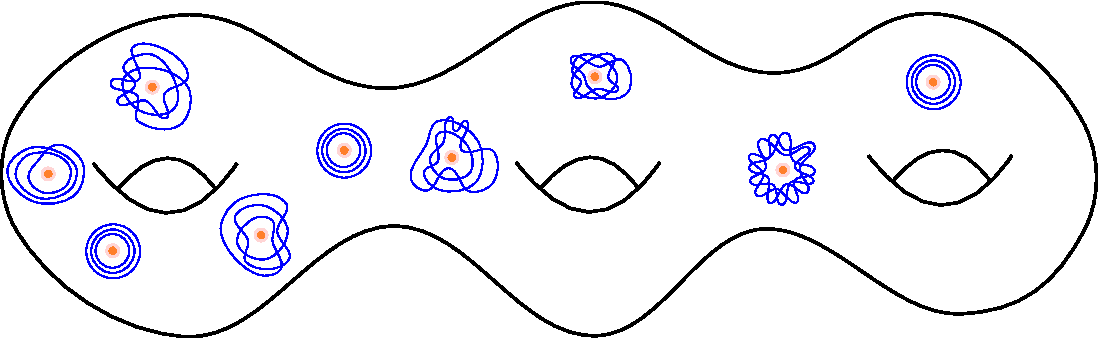
\includegraphics[scale=0.7]{figures/BettiSurface.pdf}
		\caption{An instance of a Betti surface for $\G=\SL_n$: a smooth surface with marked points endowed with the data of an $n$-stranded positive braid at each puncture. The depicted case is $n=3$. The cylindrical braid diagrams associated to these positive braid words are seen as Stokes diagrams for the local irregular data at that puncture for the irregular $\G$-local system on that surface. The case of concentric circles, i.e.~the trivial braid word, corresponds to tame behavior, whereas non-trivial positive braids lead to wild behavior.}
		\label{fig:BettiSurface}
	\end{figure}
\end{center}

\noindent {\bf Related themes for Part II.} There are different, equally interesting, research directions following the developments surveyed in these notes. A few among them are:\\

\begin{enumerate}
    \item The study of Demazure weaves $\wb$ can be understood as a generalization of the study of Betti moduli spaces for the smooth surface $S^2$ with an irregular singularity at $\infty$ whose Stokes diagram is described by the front given by the cylindrical closure of $\beta$. From that viewpoint, it is natural to explore the role of weaves through the irregular Riemann-Hilbert correspondence, and through the non-Abelian Hodge correspondence. First such steps, employing Floer theory, are established in \cite{casals2025spectralnetworksbettilagrangians}, with a focus on the non-abelianization maps and the relation to spectral networks of \cite{GNMSN,GMN14_Snakes}.\\

    More generally, the diagrammatic weave calculus exists on any smooth surface, cf.~\cite{CasalsZaslow}, and it is natural to try to extend the results for Demazure weaves and their cluster algebras to the more general context of Betti moduli spaces for Betti surfaces, as defined in \cite{casals2025spectralnetworksbettilagrangians} and see \Cref{fig:BettiSurface}. The key outstanding task is a precise generalization of the Lusztig cycles and their duals for (free) weaves on Betti surfaces. In this sense, weave calculus is particularly apt to tackle the generalization of the study of V.~Fock and A.~Goncharov for Betti surfaces with regular singularities, see e.g.~\cite{FockGoncharov09_Dilog2,FG2006,FG06a,Gon17}, or that of generic irregular data, to the case of Betti surfaces with arbitrary wild singularities. In this context, the (cylindrical closure) of the positive braid word associated to each puncture is understood as the Stokes diagram associated to the irregular data for that singularity, cf.~\cite[Section 2]{casals2025spectralnetworksbettilagrangians}.\\

    \item The additive categorification of $\Z[X(\beta)]$ using Demazure weaves, as presented in \cite{CasalsChrist}, can also be geometrically realized within the context of symplectic topology, cf.~Table \ref{tab:weaves_6D_symplectic} and \Cref{eq:NCHMS}. In this case, there is a geometric picture intertwining the symplectic topology and Lagrangian skeleta of certain Weinstein 6-manifolds, whose different flavours of Fukaya categories realize the different categories featuring in the additive categorification, and the symplectic topology of Lagrangian fillings in 4-dimensions. Details of this will appear in \cite{CasalsChrist2}.\\

    \noindent Such a geometric realization leads to a few interesting consequences. To start, using the model for additive cluster categorifications that employs the relative 3-Calabi-Yau Ginzburg dg-algebra ${\bf\Gamma}_{rel}$ of the quiver with potential $(Q_\w,W_\w)$ one obtains a series of equivalences that align with non-commutative mirror symmetry, see \Cref{eq:NCHMS}. These compare different Fukaya categories, to be understood on the A-side, to categories related to the derived category of ${\bf\Gamma}_{rel}$, which can be geometrically understood as being part of the B-side, as a form of noncommutative crepant resolution.\\

    
\small

\begin{center}
\begin{align*}
		\fbox{\xymatrix{
			&&\mathrm{per}(e\bm\Gamma_{rel}e)\cong \textcolor{purple}{\SW(F)}\ar@{=}[r]\ar@{^{(}->}[d]^{c_1}&\mathrm{per}(e\bm\Gamma_{rel}e)\cong \textcolor{purple}{\SW(F)}\ar@{^{(}->}[d]^{c_2}\\
			\mathrm{pvd}_{e}(\bm\Gamma_{rel})\cong \textcolor{purple}{\mathcal{F}(Y)\quad}\ar@{^{(}->}^{i_1}"2,3"\ar@{->}_{\cong}[d]^{j}&&\mathrm{per}(\bm\Gamma_{rel})\cong\textcolor{purple}{\SW(Y,F)}\ar[r]^{p_1}\ar@{->>}[d]^{q_1}&\mathcal{C}(Q,F,W)\cong\textcolor{purple}{\mathcal{N}(Y,F)}\ar@{->>}[d]^{q_2}\\
			\mathrm{pvd}({\bm\Gamma}(\overline{Q},\overline{W}))\cong \textcolor{purple}{\mathcal{F}(Y)\quad}\ar@{^{(}->}^{i_2}"3,3"&&\mathrm{per}({\bm\Gamma}(\overline{Q},\overline{W}))\cong\textcolor{purple}{\SW(Y)}\ar[r]^{p_2}&\mathcal{C}(\overline{Q},\overline{W})\cong \textcolor{purple}{\RW(Y)}
		}}
\end{align*}\captionof{figure}{A diagram relating categories built from the relative 3-Calabi-Yau Ginzburg dg-algebra ${\bf\Gamma}_{rel}$, in black, and their symplectic geometric realizations, employing flavours of Fukaya categories, in red.\\}
    \label{eq:NCHMS}
\end{center}
\normalsize

    \item To our knowledge, it remains an interesting question to construct a symplectic topological realization of the monoidal categorifications in \cite{KKOP2025MonoidalIII}, perhaps starting with a symplectic geometric realization of the Hernandez-Leclerc category and the associated braid group symmetries. Their direct relation to modules over KLR algebras and, in turn, the realization of such algebras in terms of endomorphisms of certain perverse sheaves, are first hints towards the fact that a symplectic geometric realization likely should exist.\\

    \item Similarly, many of the results connecting symplectic topology and cluster algebras, some illustrated in these notes, hint toward a well-structured theory of {\it positive} symplectic topology. It would be enlightening to better formalize how such positive properties of algebraic invariants arising in Floer theory (or microlocal sheaf theory) can be justified geometrically. For instance, one could seek a natural geometric explanation for the semi-twist functors.\\

    \item Finally, at least for $\G=\SL_n$, the symplectic topological constructions provide algebraic structures much richer than a commutative algebra, including noncommutative versions of braid varieties, parabolic ones, and $A_\infty$ or dg categories for which $X(\beta)$ appears as part of the moduli of pseudoperfect objects. There is not yet a completely agreed upon notion of non-commutative cluster algebra, or the notion of a cluster derived stack, or the concept of a cluster $A_\infty$ or dg category, so that their pseudoperfect moduli stack is a cluster derived stack. That said, as a personal view, any of the Legendrian dg algebra $\mathbb{A}(\La_\beta)$, or its dg category of perfect modules, or equivalently the partially wrapped Fukaya category of $\La_\beta$, or the dg category of sheaves in $\R^2$ with singular support in $\La_\beta$, should be salient examples of these to-be-defined more general notions of being cluster.\\
\end{enumerate}
\normalsize

We conclude with an explanation of the concepts featuring in \Cref{eq:NCHMS}. The black part of the diagram (the left hand side of the equivalences) focuses on the representation theory of the relative Ginzburg dg-algebra $\bm\Gamma_{rel}:=\bm\Gamma_{rel}(Q,W)$, which could be understood as a form of non-commutative crepant resolution on the $B$-side of this non-commutative form of homological mirror symmetry. Here $e\in \bm\Gamma_{rel}$ is the frozen idempotent, $\bm\Gamma(\overline{Q},\overline{W})$ is the absolute CY3 Ginzburg dg-algebra, $\mathcal{C}(Q,F,W)$ the relative cluster category and $\mathcal{C}(\overline{Q},\overline{W})$ the absolute cluster category, cf.~\cite{amiot2011generalizedclustercategories,MR4581969,KellerWu2023Higgs}. The red part of the diagram (the right hand side of the equivalences) focuses on categorical symplectic invariants of the Weinstein 6-manifold $Y=(Y_\w,\la_\w)$ and its associated Lefschetz fibration $\pi:(Y_\w,\la_\w)\lr\cC$, where $F:=F_\pi$ denotes a regular fiber, which is a 4-dimensional Weinstein subdomain. In this viewpoint, the Demazure weave $\w$ can be understood as a form of branch cut for the Lefschetz fibration $\pi$: while a rather excessive one, it is provably useful in structuring many of the symplectic objects involved in the study of $Y=(Y_\w,\la_\w)$.\\

It is important to emphasize that this 6-manifold $(Y_\w,\la_\w)$ also admits a geometric description as a $T^*S^1$-branched cover of $(\C^2,\la_\std)$ branched along the symplectic push-off of $L_\w$. Since the symplectic push-offs of any Demazure weaves $\w:\beta\lr\delta(\beta)$ are symplectically isotopic, the symplectomorphism type of $(Y_\w,\la_\w)$ is independent of $\w$. (From the Lefschetz fibration viewpoint, this can be argued via Hurwitz moves.) This geometric model factoring through 4-dimensions also explains geometrically why these Fukaya categories in 6-dimensions actually additively categorify the cluster algebra associated to the 4-dimensional framework, whose clusters are given by Lagrangian fillings. This 6-dimensional red part of the diagram can be understood as the $A$-side and, quite coarsely put, the cluster varieties extracted from the 4-dimensional setting are closely related (degenerate) to the space of stability conditions of the Fukaya-Seidel category of such $(Y_\w,\la_\w)$. About the red part of the diagram:\\

\begin{enumerate}
    \item (Middle column) The functor $c_1:\SW(F)\lr\SW(Y,F)$ is the Orlov cup functor between the wrapped Fukaya category of $F$, and the partially wrapped Fukaya category of $Y$ with a stop at $F$, which is equivalent to the Fukaya-Seidel category of $\pi$. See e.g.~\cite[Section 2.4]{Syl19}, \cite[Section 3.5]{GPSCV} and \cite[Example 1.23]{GPS18}. The functor $q_1:\SW(Y,F)\lr\SW(Y)$ is the stop removal (pushforward) functor, cf.~\cite[Theorem 1.20]{GPS18}.\\

    \item (Bottom row) The Rabinowitz wrapped Fukaya category $\RW(Y)$ is constructed in \cite[Section 4]{ganatra2022rabinowitzfukayacategoriescategorical}. By \cite[Theorem 1.1]{ganatra2022rabinowitzfukayacategoriescategorical}, it is equivalent to the formal punctured neighborhood of infinity of $\SW(Y)$, and the functor $p_2:\SW(Y)\lr \RW(Y)$ is given in \cite[Lemma 4.11]{ganatra2022rabinowitzfukayacategoriescategorical}. Note that $\RW(Y)$ is an absolute smooth 2-Calabi-Yau category, cf.~\cite[Theorem 1.2.(1)]{bae2024calabiyaustructuresrabinowitzfukaya}, as it should be according to the theory of additive cluster categorifications, cf.~e.g.~\cite[Sections 2\&3]{amiot2011generalizedclustercategories}. The natural inclusion functor $i_2:\mathcal{F}(Y)\lr\SW(Y)$ gives the proper subcategory (of closed compact Lagrangians) of the smooth category $\SW(Y)$, and exactness of the bottom row follows from \cite[Corollary 1.4]{ganatra2022rabinowitzfukayacategoriescategorical}.\\
    
    \item (Right column \& Middle row) The category $\mathcal{N}(Y,F)$ is introduced in \cite[Section 3.5]{gao2024fukayaainfinitystructurenear}, where it is referred to as the negatively wrapped Fukaya category, cf.~also \cite[Section 5]{seidel2025fukayaainftystructuresassociatedlefschetz}. Since $F$ is a full stop, \cite[Theorem 1.1.(ii)]{gao2024fukayaainfinitystructurenear} implies that $\mathcal{N}(Y,F)$ is equivalent to the formal completion of $\SW(Y,F)$ along the subcategory given by the image of $\SW(F)$ under the cup functor. The cup functor thus descends to $c_2:\SW(F)\lr\mathcal{N}(Y,F)$ and the pushforward functor $q_2:\mathcal{N}(Y,F)\lr\RW(Y)$ is given by \cite[Theorem 1.5]{gao2024fukayaainfinitystructurenear}, as $\RW(Y)\cong \mathcal{N}(Y,\emptyset)$. Exactness of the right column follows from \cite[Corollary 1.2]{gao2024fukayaainfinitystructurenear}. Similarly, for the middle row, $p_1:\SW(Y,F)\lr\mathcal{N}(Y,F)$ is given by \cite[(1.12)]{gao2024fukayaainfinitystructurenear}.
\end{enumerate}
\tiny
\begin{center}
\begin{table}
\centering
  \caption{A summary of the key objects featuring in the symplectic geometric realization of the additive cluster categorification of $\Z[X(\beta)]$ via weaves, cf.~\cite{CasalsChrist,CasalsChrist2}, and their relation to the viewpoint presented in these notes, which is focused on Lagrangian fillings in 4-dimensions.}
  \label{tab:weaves_6D_symplectic}
\qquad\begin{tabular}{ |P{3cm}|P{4cm}|P{3cm}|P{3.5cm}|P{3.5cm}|}
	\hline
    
	{\bf Demazure weaves $\w$} & {\bf Sympl.~Topology in $T^*\mathbb{R}^2$} & {\bf $\mbox{Perf}(A_\beta)$ - Rel.~CY2} & {\bf Symplectic 6-folds} & {\bf $R\Gamma(\mathcal{F}_\w)$ - Relative CY3}\\
	\hline
    
	Boundary braid $\beta=\dd\w$ ($\tt$-based) & Legendrian Link $\Lambda_\beta\subseteq T^*_\infty\mathbb{R}^2$ ($\tt$-based, e.g.~Stokes diagram) & Braid variety $X(\beta)$ from Leg.~dg algebra $\mathbb{A}_\beta$ & Liouville sector $(Y^6,F^4)$, $F\cong A_n\mbox{-plumbing of } T^*S^2$ & Relative CY3 category $R\Gamma(\mathcal{F}_\w)$ - saturated\\
	% & (with marked points $T$) & \\
	\hline
    
	Demazure weave $\w:\beta\to\delta(\beta)$ &  Exact Lagrangian filling $L_\w$ of $\La_\beta$ ($\w$ describes front) & Open toric chart $T_L=(\mathbb{C}^\times)^{d}\subseteq X(\beta)$ & Lefschetz fibration $\pi:Y\stackrel{F}{\lr}\cC$ & Exceptional collection of thimbles in $R\Gamma(\mathcal{F}_\w)$\\
	\hline

    Lusztig cycle $\g_i$ on $\w$ (tropical propagation) & Lagrangian disk $D_i\sse T^*\R^2$ with boundary on Lagrangian $L$ & Cluster $\SX$-coordinate as $\dd D_i$-monodromy & Skeleton component (e.g.~Lagrangian $S^3$) & Categorical Lusztig cycle (object of $R\Gamma(\mathcal{F}_\w)$)\\
	
	\hline
    
	  Lusztig cycles & $\lL$-compressing system  & Cluster $\SX$-coordinates & Lagrangian skeleton & Simple-minded collection\\
	
	\hline
    
	Dual Lusztig cycles & Dual $\lL$-compressing system & Cluster $\SA$-coordinates & Cocores of skeleton & Silting collection\\
	
	\hline

%	\hline
    
    
	Intersections $\g_i\cap\g_j$ & Intersections of $\dd D_i,\dd D_j$ & Quiver in seed for $X(\beta)$ & Lagr.~intersections & Ext groups \\
	\hline

    Weave potential $W_\w$, via planar regions & $A_\infty$-structure on symplectic push-off $S(L_\w)$ of $L_\w$ & Rigid QP $(Q_\w,W_\w)$ for $\Z[X(\beta)]$ & $A_\infty$-structure in $Y^6$ (e.g.~between 3-spheres) & formal completion along $\mathcal{D}$ as relative cluster category \\

    \hline
\end{tabular}
\end{table}
\end{center}
\normalsize

Similar to Part I, the study of symplectic topological objects associated to $\beta$ and its Demazure weaves seems to provide fertile ground for new insights and ideas, as hopefully illustrated by the instances above. From this viewpoint, we hope that the explicit diagrammatic calculus of weaves and its developing theory can continue to help us enjoy the wonders of contact and symplectic topology, providing new understanding and results within the field, and also bridging across to different areas of mathematics.\\

%%%%%%%%%%%%%%%%%%%%%%%%%%%%%%%%%%%%%
%%%%%%%%%%%%%%%%%%%%%%%%%%%%%%%%%%%%%
%%%%%%%%%%%%%%%%%%%%%%%%%%%%%%%%%%%%%
\noindent {\bf Acknowledgments}: I want to thank the organizers of the Current Developments in Mathematics conference for their invitation. I am also grateful to my coauthors in \cite{CasalsZaslow,CGGLSS25,CasalsChrist,casals2023demazureweavesreducedplabic,CasalsLi24} for valuable discussions. Special thanks are due to J.~Etnyre, H.~Gao, L.~Ng, Y.~J.~Nho and D.~Weng, whose savoir-faire, ideas and support are a source of professional joy. The author is supported by the National Science Foundation under the grant DMS-2505760.\sbs\\

%%%%%%%%%%%%%%%%%%%%%%%%%%%%%%%%%%%%%
%%%%%%%%%%%%%%%%%%%%%%%%%%%%%%%%%%%%%
%%%%%%%%%%%%%%%%%%%%%%%%%%%%%%%%%%%%%

\noindent {\bf Conventions}: The base ring throughout the notes is $\kk=\Z$. In Part II, we have focused on geometric realization of parts of Part I using Floer theory, specifically through the use of the Legendrian dg algebra and Reeb chords. A similar description exists from the viewpoint of the microlocal theory of sheaves, see e.g.~\cite{CasalsZaslow,CasalsWeng22,casals2023demazureweavesreducedplabic}.\sbs\\

%%%%%%%%%%%%%%%%%%%%%%%%%%%%%%%%%%%%%
%%%%%%%%%%%%%%%%%%%%%%%%%%%%%%%%%%%%%
%%%%%%%%%%%%%%%%%%%%%%%%%%%%%%%%%%%%%
\noindent {\bf A comment on references}: Part I articulates many ideas implicit in \cite{CasalsZaslow,CasalsWeng22} and \cite{CGGLSS25}. That said, in order to favor conceptual clarity, the choice of presentation differs from \cite{CGGLSS25}. In particular, I have emphasized the role and importance of dual Lusztig cycles throughout the manuscript and clarified the construction of cluster $\SA$-variables in terms of them. Many of the facts surveyed in this article can be rigorously deduced from the available literature; the few that require more serious work are currently being written up.\sbs
